\documentclass[tikz,border=3mm]{standalone}
\usepackage{fontspec}
\usepackage{amsmath}
\usepackage{xcolor}
\usepackage{tikz}
\usetikzlibrary{arrows.meta,calc,decorations.pathreplacing,backgrounds,shapes.geometric,shapes.symbols,patterns.meta}
\setmainfont{Comic Sans MS}

\definecolor{nvgreen}{HTML}{76B900}
\definecolor{nvdark}{HTML}{1A1A1A}
\definecolor{nvgraphite}{HTML}{36393B}
\definecolor{nvpale}{HTML}{EDF7DA}
\definecolor{nvsoft}{HTML}{F6F8F3}
\definecolor{nvline}{HTML}{C9D0C2}
\definecolor{emerald}{HTML}{0B6B45}
\definecolor{teal}{HTML}{087F8C}
\definecolor{amber}{HTML}{F2A900}
\definecolor{mint}{HTML}{E7F5EE}
\definecolor{ivory}{HTML}{FBFCF7}
\definecolor{darkpanel}{HTML}{171A18}
\definecolor{darklane}{HTML}{5E665F}
\definecolor{cyanaccent}{HTML}{35C4B5}

\tikzset{
  >={Stealth[length=2.3mm,width=1.7mm]},
  ctitle/.style={font=\fontsize{15}{17}\selectfont,align=center},
  csub/.style={font=\fontsize{8}{10}\selectfont,align=center},
  clabel/.style={font=\fontsize{8}{9.5}\selectfont,align=center},
  ctiny/.style={font=\fontsize{6.4}{7.6}\selectfont,align=center},
  cmicro/.style={font=\fontsize{5.3}{6.3}\selectfont,align=center}
}

\begin{document}
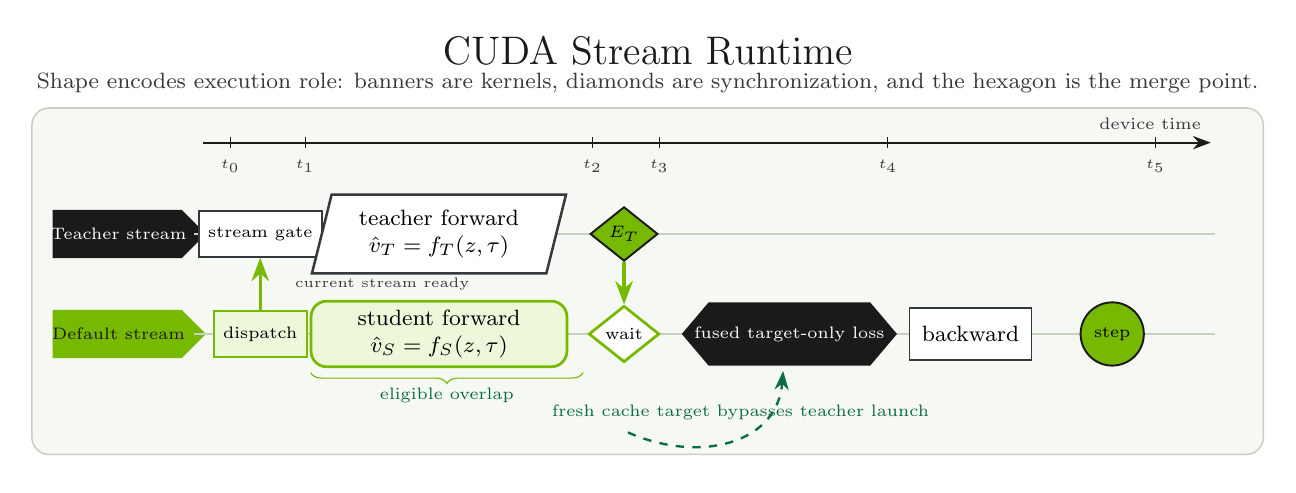
\begin{tikzpicture}[x=1cm,y=1cm]
  \node[ctitle,text=nvdark] at (8,5.55) {CUDA Stream Runtime};
  \node[csub,text=nvgraphite] at (8,5.14)
    {Shape encodes execution role: banners are kernels, diamonds are synchronization, and the hexagon is the merge point.};

  \fill[rounded corners=2.2mm,fill=nvsoft,draw=nvline,line width=.55pt]
    (.18,.42) rectangle (15.82,4.82);
  \draw[-Stealth,draw=nvdark,line width=.75pt] (2.35,4.38) -- (15.15,4.38);
  \node[ctiny,text=nvgraphite,anchor=east] at (15.15,4.62) {device time};
  \foreach \x/\t in {2.70/$t_0$,3.65/$t_1$,7.30/$t_2$,8.15/$t_3$,11.05/$t_4$,14.45/$t_5$} {
    \draw[draw=nvdark,line width=.4pt] (\x,4.31) -- (\x,4.45);
    \node[cmicro,text=nvgraphite] at (\x,4.08) {\t};
  }

  \path[fill=nvdark,draw=nvdark]
    (.45,2.92) -- (2.08,2.92) -- (2.38,3.22) -- (2.08,3.52) -- (.45,3.52) -- cycle;
  \node[ctiny,text=white] at (1.28,3.22) {Teacher stream};
  \path[fill=nvgreen,draw=nvgreen]
    (.45,1.65) -- (2.08,1.65) -- (2.38,1.95) -- (2.08,2.25) -- (.45,2.25) -- cycle;
  \node[ctiny,text=nvdark] at (1.28,1.95) {Default stream};
  \draw[draw=nvline,line width=.55pt] (2.24,3.22) -- (15.20,3.22);
  \draw[draw=nvline,line width=.55pt] (2.24,1.95) -- (15.20,1.95);

  \node[rectangle,fill=white,draw=nvgraphite,line width=.7pt,ctiny,
        minimum width=1.05cm,minimum height=.58cm] (gate) at (3.08,3.22) {stream gate};
  \node[trapezium,trapezium left angle=76,trapezium right angle=104,
        fill=white,draw=nvgraphite,line width=.9pt,clabel,
        minimum width=3.25cm,minimum height=.70cm] (teacher) at (5.35,3.22)
    {teacher forward\\$\hat v_T=f_T(z,\tau)$};
  \node[diamond,aspect=1.25,fill=nvgreen,draw=nvdark,line width=.7pt,
        ctiny,inner sep=1.5pt] (record) at (7.70,3.22) {$E_T$};

  \node[rectangle,fill=nvpale,draw=nvgreen,line width=.8pt,ctiny,
        minimum width=1.05cm,minimum height=.58cm] (dispatch) at (3.08,1.95) {dispatch};
  \node[rectangle,rounded corners=2mm,fill=nvpale,draw=nvgreen,line width=1pt,clabel,
        minimum width=3.25cm,minimum height=.72cm] (student) at (5.35,1.95)
    {student forward\\$\hat v_S=f_S(z,\tau)$};
  \node[diamond,aspect=1.25,fill=white,draw=nvgreen,line width=1pt,
        ctiny,inner sep=1.5pt] (wait) at (7.70,1.95) {wait};
  \path[fill=nvdark,draw=nvdark,line width=.7pt]
    (8.45,1.95) -- (8.78,2.34) -- (10.82,2.34) -- (11.15,1.95) --
    (10.82,1.56) -- (8.78,1.56) -- cycle;
  \node[ctiny,text=white] at (9.80,1.95) {fused target-only loss};
  \node[rectangle,fill=white,draw=nvgraphite,line width=.7pt,clabel,
        minimum width=1.55cm,minimum height=.65cm] (back) at (12.10,1.95) {backward};
  \node[circle,fill=nvgreen,draw=nvdark,line width=.7pt,ctiny,
        minimum size=.78cm] at (13.90,1.95) {step};

  \draw[-Stealth,draw=nvgreen,line width=1.2pt] (dispatch.north) -- (gate.south);
  \node[cmicro,text=nvgraphite,anchor=west] at (3.40,2.58) {current stream ready};
  \draw[-Stealth,draw=nvgreen,line width=1.2pt] (record.south) -- (wait.north);
  \draw[decorate,decoration={brace,mirror,amplitude=4pt},draw=nvgreen]
    (3.72,1.46) -- (7.18,1.46);
  \node[ctiny,text=emerald] at (5.45,1.17) {eligible overlap};

  \draw[-Stealth,dashed,draw=emerald,line width=.85pt]
    (7.75,.70) .. controls (8.65,.30) and (9.65,.55) .. (9.72,1.48);
  \node[ctiny,text=emerald] at (9.18,.96)
    {fresh cache target bypasses teacher launch};
\end{tikzpicture}
\end{document}
